\chapter{Capacidad de distinción de las métricas}\label{sec:diferencias}
\addcontentsline{toc}{chapter}{Capacidad de distinción de las métricas}

En este capítulo se realizarán una serie de estudios estadísticos que muestran la capacidad de todas y cada una de las métricas para diferenciar entre los grupos de prácticas en riesgo y los que no tienen problemas para resolver los retos propuestos por el profesorado de la asignatura.

Para analizar la capacidad de distinción de una métrica se procederá, tras eliminar sus posibles valores extremos, a separar sus valores en dos poblaciones según correspondan a grupos \emph{``LOW''} o \emph{``GOOD''} y a realizar el test de Welch con la finalidad de dilucidar si tienen medias iguales.

\subsection{Estudio de la capacidad de separación de las medidas clásicas del rendimiento}

\subsection{Estudio de la capacidad de separación de las medidas de complejidad de propósito general}

Como podemos ver en la Figura \ref{fig:tstudentcomplexity}, la única medida con medias estadísticamente diferentes en ambas poblaciones es \emph{We} ($p-value = 0.02562 < 0.05$). Podríamos igualmente considerar que hay diferencias significativas entre las medias de la medida \emph{Ef}, aunque con un grado de certeza menor ($p-value = 0.1696 < 0.2$). Adicionalmente, podemos ver las funciones de densidad de las dos poblaciones de cada métrica en la Figura \ref{fig:tstudentcomplexitydensity}.

\begin{figure}[H]
\centering
\begin{tikzpicture}
  \node[inner sep=0pt] (image1) at (0,0)
    {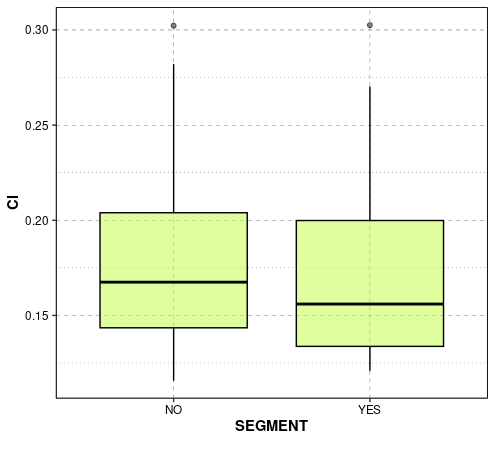
\includegraphics[width=0.3\textwidth]{diferencias/cl.png}};
  \node[below, align=center, text width=0.3\textwidth] at (image1.south)
    {\scriptsize\textcolor{gray}{\texttt{t = 0.053933, df = 13.459,} \texttt{p-value = 0.9578}}};
\end{tikzpicture}%
\begin{tikzpicture}
  \node[inner sep=0pt] (image2) at (0,0)
    {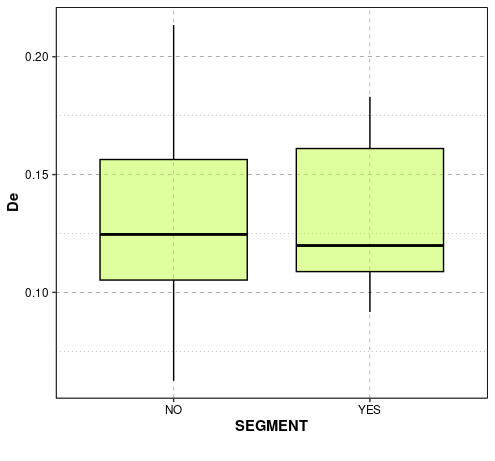
\includegraphics[width=0.3\textwidth]{diferencias/de.png}};
  \node[below, align=center, text width=0.3\textwidth] at (image2.south)
    {\scriptsize\textcolor{gray}{\texttt{t = -0.022254, df = 18.067,} \texttt{p-value = 0.9825}}};
\end{tikzpicture}%
\begin{tikzpicture}
  \node[inner sep=0pt] (image3) at (0,0)
    {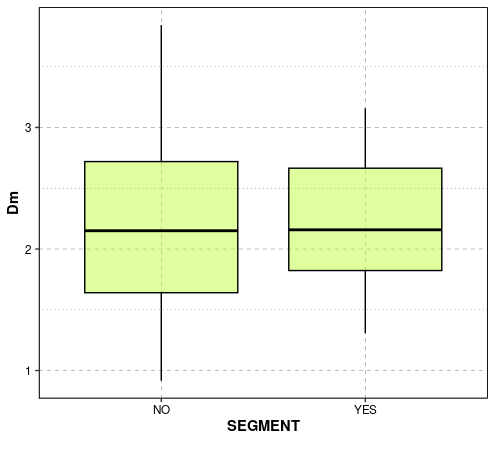
\includegraphics[width=0.3\textwidth]{diferencias/dm.png}};
  \node[below, align=center, text width=0.3\textwidth] at (image3.south)
    {\scriptsize\textcolor{gray}{\texttt{t = 0.074065, df = 17.648,} \texttt{p-value = 0.9418}}};
\end{tikzpicture}%

\begin{tikzpicture}
  \node[inner sep=0pt] (image4) at (0,0)
    {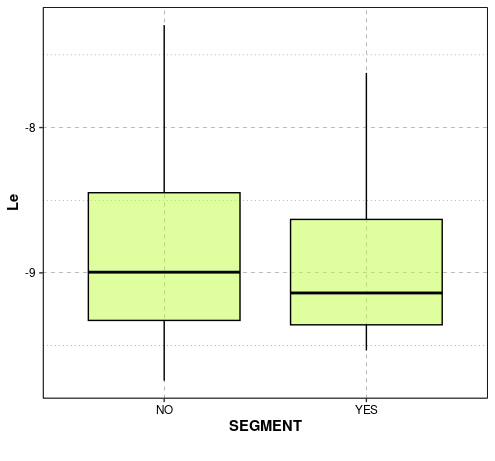
\includegraphics[width=0.3\textwidth]{diferencias/le.png}};
  \node[below, align=center, text width=0.3\textwidth] at (image4.south)
    {\scriptsize\textcolor{gray}{\texttt{t = -0.4641, df = 16.403,} \texttt{p-value = 0.6487}}};
\end{tikzpicture}%
\begin{tikzpicture}
  \node[inner sep=0pt] (image5) at (0,0)
    {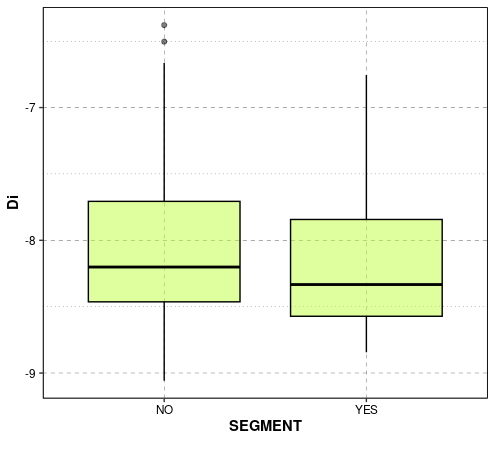
\includegraphics[width=0.3\textwidth]{diferencias/di.png}};
  \node[below, align=center, text width=0.3\textwidth] at (image5.south)
    {\scriptsize\textcolor{gray}{\texttt{t = -0.53037, df = 16.28,} \texttt{p-value = 0.603}}};
\end{tikzpicture}%
\begin{tikzpicture}
  \node[inner sep=0pt] (image6) at (0,0)
    {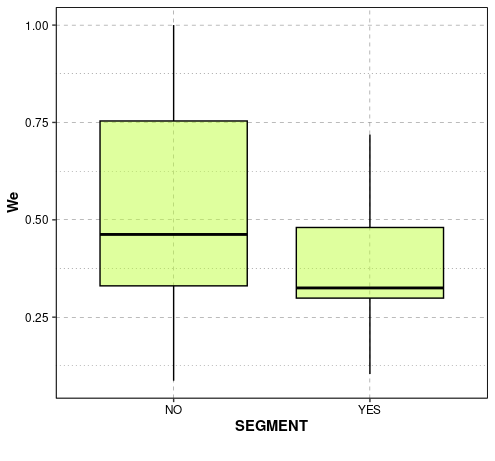
\includegraphics[width=0.3\textwidth]{diferencias/we.png}};
  \node[below, align=center, text width=0.3\textwidth] at (image6.south)
    {\scriptsize\textcolor{gray}{\texttt{t = -2.3903, df = 22.496,} \texttt{p-value = 0.02562}}};
\end{tikzpicture}%

\begin{tikzpicture}
  \node[inner sep=0pt] (image7) at (0,0)
    {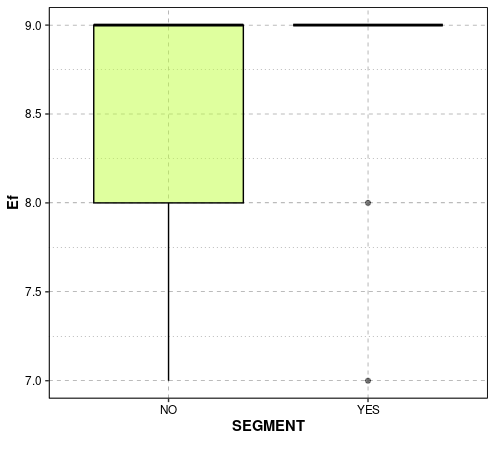
\includegraphics[width=0.3\textwidth]{diferencias/ef.png}};
  \node[below, align=center, text width=0.3\textwidth] at (image7.south)
    {\scriptsize\textcolor{gray}{\texttt{t = 1.4405, df = 15.538,} \texttt{p-value = 0.1696}}};
\end{tikzpicture}%
\begin{tikzpicture}
  \node[inner sep=0pt] (image8) at (0,0)
    {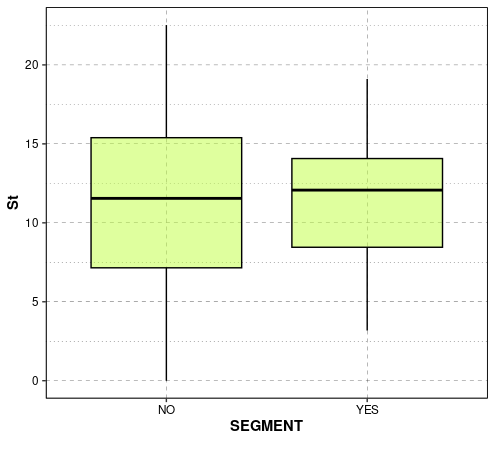
\includegraphics[width=0.3\textwidth]{diferencias/st.png}};
  \node[below, align=center, text width=0.3\textwidth] at (image8.south)
    {\scriptsize\textcolor{gray}{\texttt{t = 0.15625, df = 17.012,} \texttt{p-value = 0.8777}}};
\end{tikzpicture}%
\begin{tikzpicture}
  \node[inner sep=0pt] (image9) at (0,0)
    {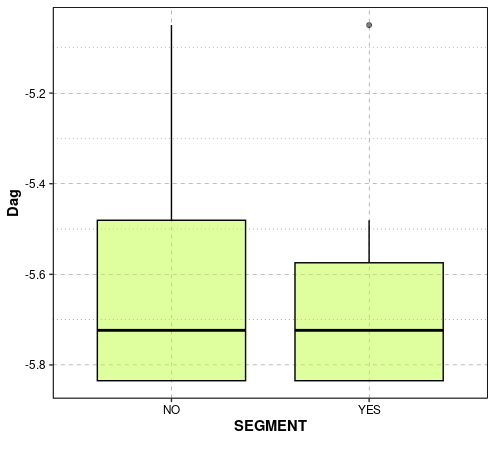
\includegraphics[width=0.3\textwidth]{diferencias/dag.png}};
  \node[below, align=center, text width=0.3\textwidth] at (image9.south)
    {\scriptsize\textcolor{gray}{\texttt{t = -0.23354, df = 14.668,} \texttt{p-value = 0.8186}}};
\end{tikzpicture}%

\begin{tikzpicture}
  \node[inner sep=0pt] (image10) at (0,0)
    {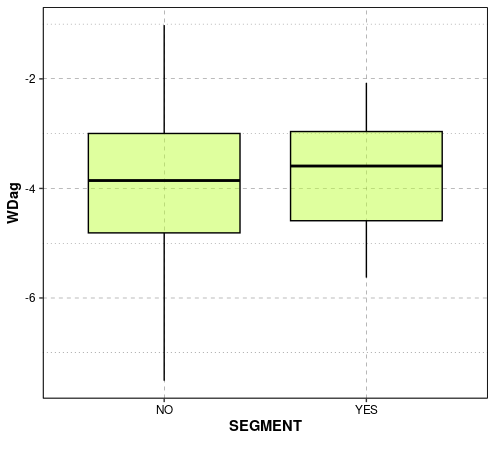
\includegraphics[width=0.3\textwidth]{diferencias/wdag.png}};
  \node[below, align=center, text width=0.3\textwidth] at (image10.south)
    {\scriptsize\textcolor{gray}{\texttt{t = 0.38716, df = 18.254,} \texttt{p-value = 0.7031}}};
\end{tikzpicture}%
\begin{tikzpicture}
  \node[inner sep=0pt] (image11) at (0,0)
    {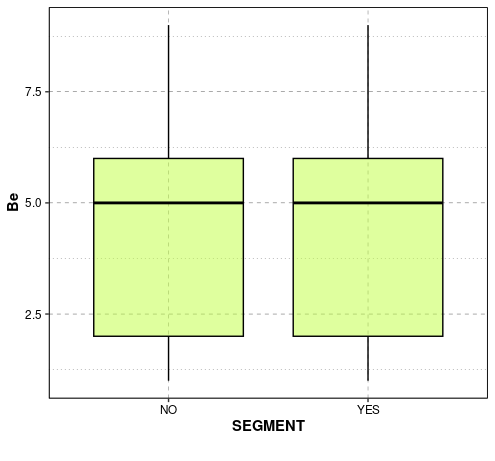
\includegraphics[width=0.3\textwidth]{diferencias/be.png}};
  \node[below, align=center, text width=0.3\textwidth] at (image11.south)
    {\scriptsize\textcolor{gray}{\texttt{t = -0.044943, df = 15.542,} \texttt{p-value = 0.9647}}};
\end{tikzpicture}%
\begin{tikzpicture}
  \node[inner sep=0pt] (image12) at (0,0)
    {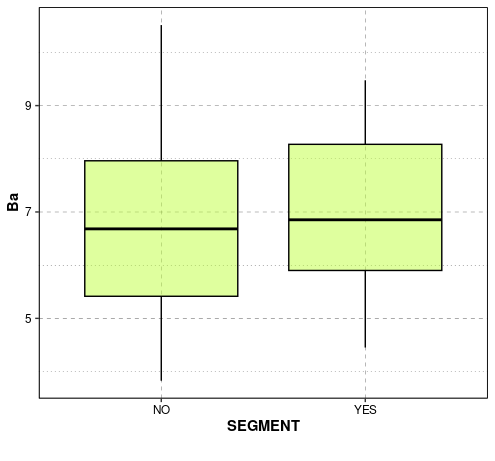
\includegraphics[width=0.3\textwidth]{diferencias/ba.png}};
  \node[below, align=center, text width=0.3\textwidth] at (image12.south)
    {\scriptsize\textcolor{gray}{\texttt{t = 0.29811, df = 15.431,} \texttt{p-value = 0.7696}}};
\end{tikzpicture}%

\caption{Boxplots de las diferentes medidas de complejidad por grupos de alumnos.}
\label{fig:tstudentcomplexity}
\end{figure}

\begin{figure}[H]
\centering
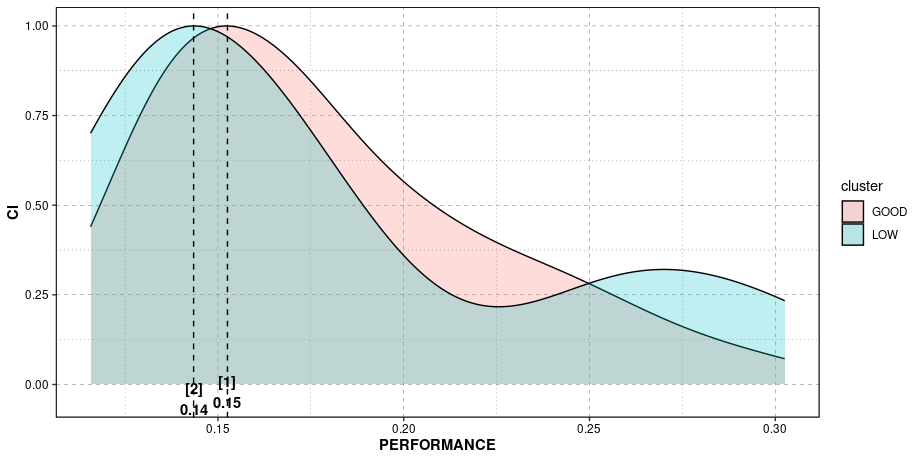
\includegraphics[width=0.48\textwidth]{diferencias/densitycl.png}
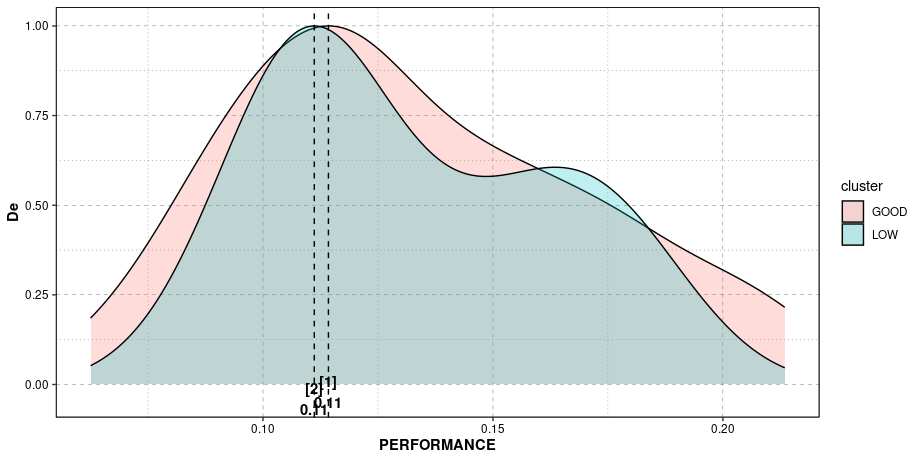
\includegraphics[width=0.48\textwidth]{diferencias/densityde.png} \\
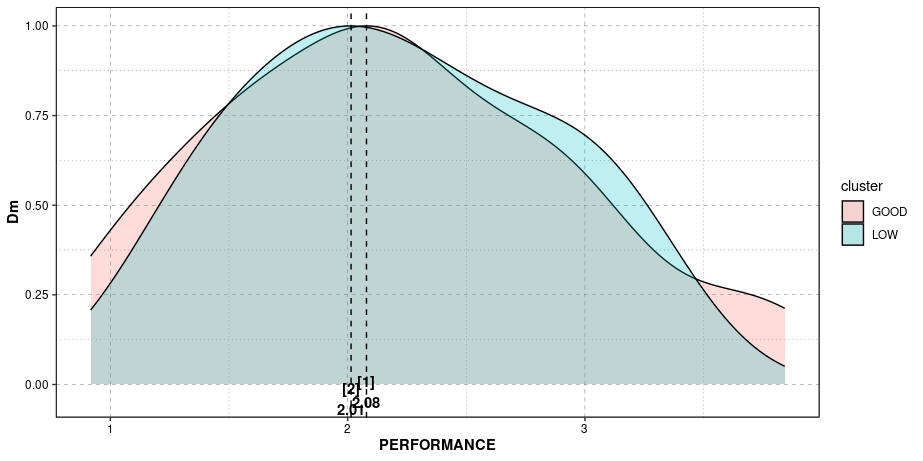
\includegraphics[width=0.48\textwidth]{diferencias/densitydm.png}
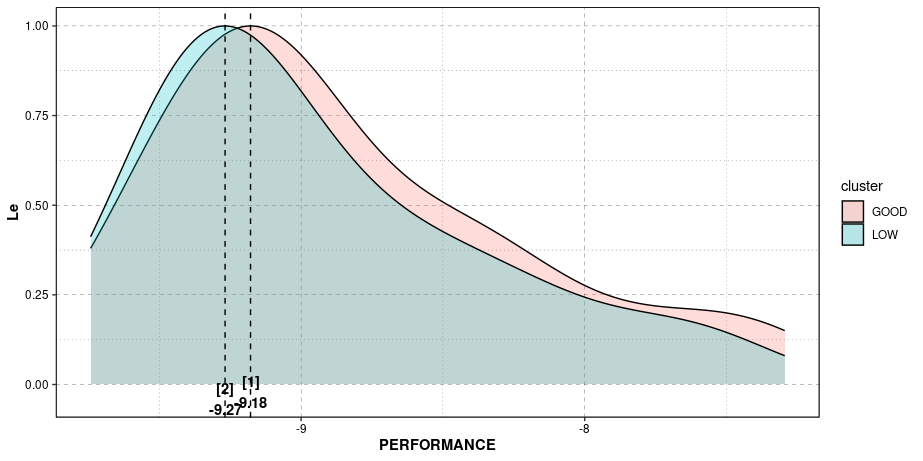
\includegraphics[width=0.48\textwidth]{diferencias/densityle.png} \\
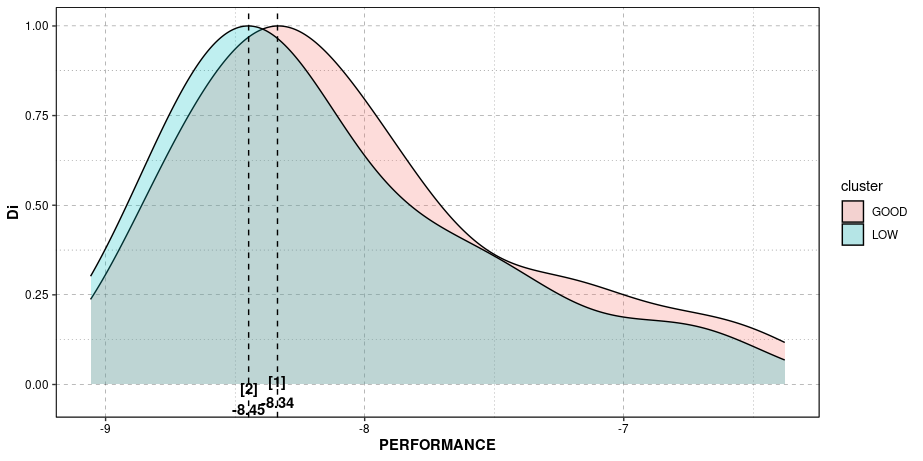
\includegraphics[width=0.48\textwidth]{diferencias/densitydi.png}
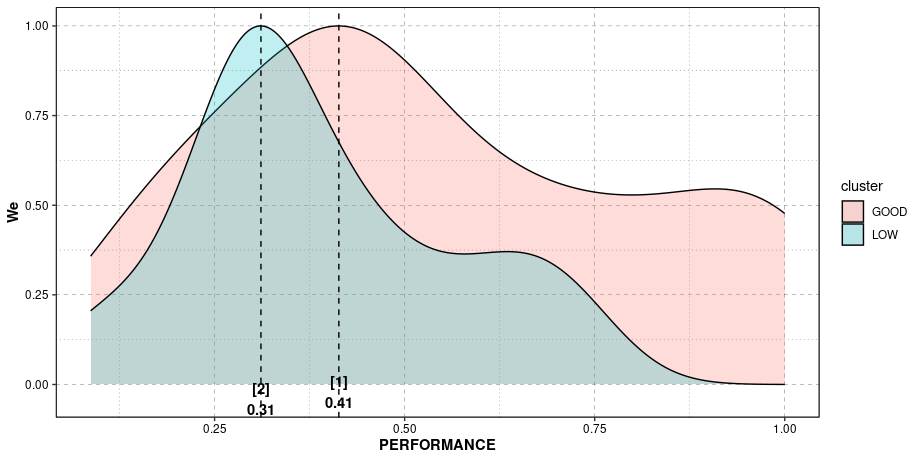
\includegraphics[width=0.48\textwidth]{diferencias/densitywe.png} \\
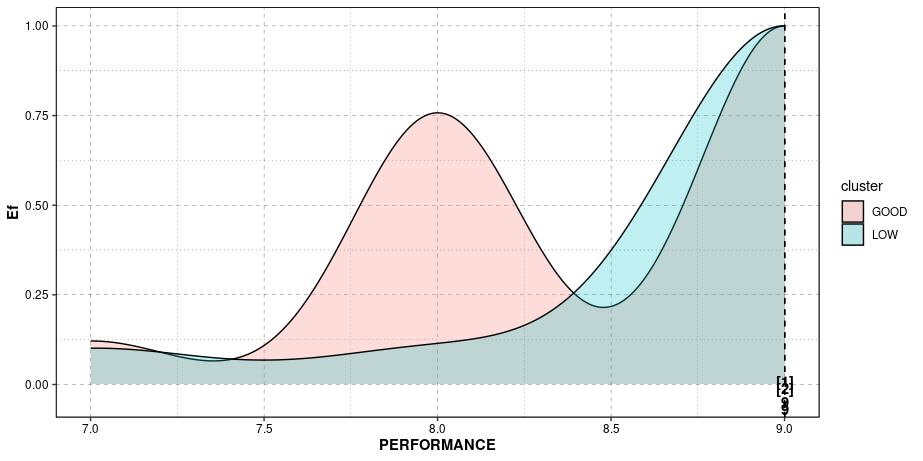
\includegraphics[width=0.48\textwidth]{diferencias/densityef.png}
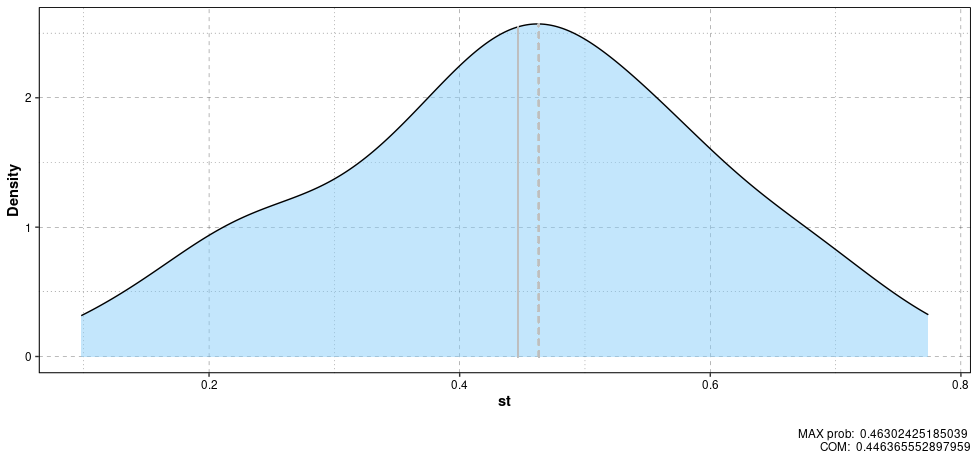
\includegraphics[width=0.48\textwidth]{diferencias/densityst.png} \\
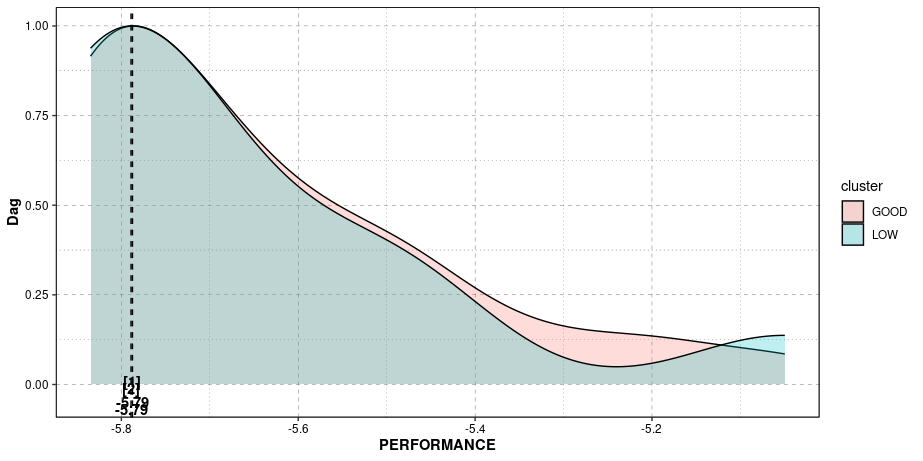
\includegraphics[width=0.48\textwidth]{diferencias/densitydag.png}
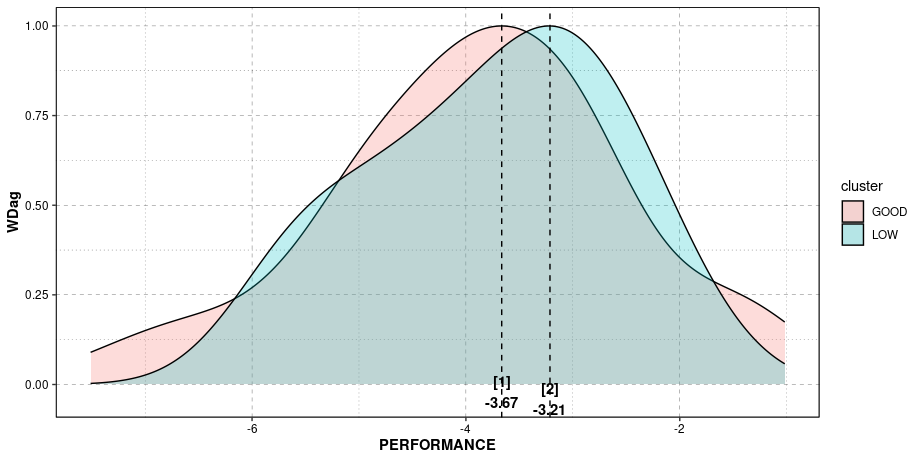
\includegraphics[width=0.48\textwidth]{diferencias/densitywdag.png} \\
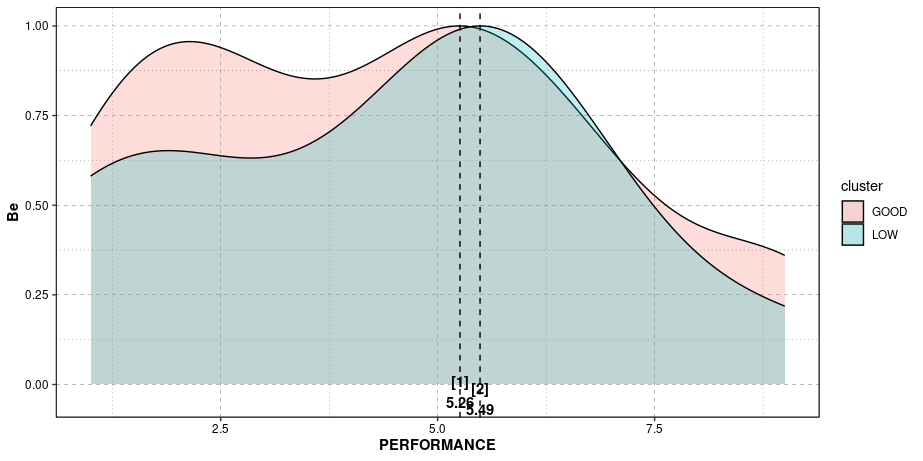
\includegraphics[width=0.48\textwidth]{diferencias/densitybe.png}
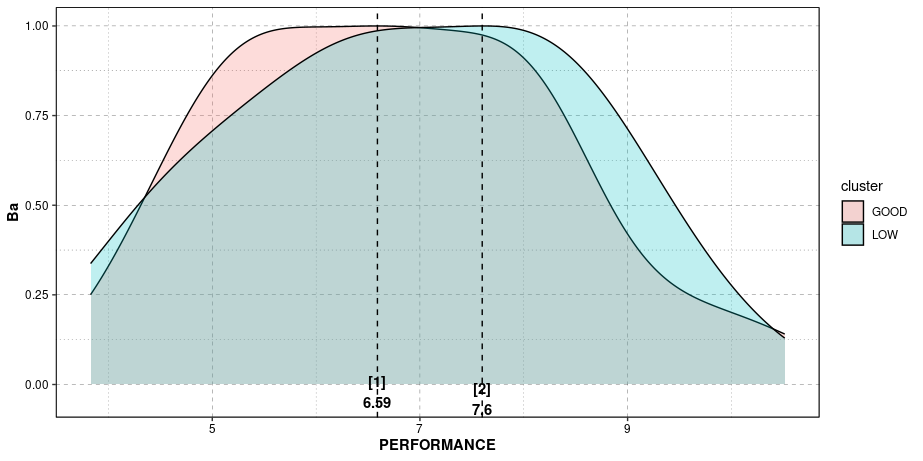
\includegraphics[width=0.48\textwidth]{diferencias/densityba.png}
\caption{Funciones de densidad de las diferentes medidas de complejidad por grupos de alumnos.}
\label{fig:tstudentcomplexitydensity}
\end{figure}

